\begin{activity} \label{A:9.7.7} 
Suppose a moving object in space has its velocity given by
\[\vv(t) = (-2\sin(2t)) \vi + (2 \cos(t)) \vj + \left(1 - \frac{1}{1+t}\right) \vk.\]
A graph of the position of the object for times $t$ in $[-0.5,3]$ is shown in Figure \ref{F:9.7.VVD_Example}.  Suppose further that the object is at the point $(1.5,-1,0)$ at time $t=0$. 
	\ba
	\item Determine $\va(t)$, the acceleration of the object at time $t$.

	\item Determine $\vr(t)$, position of the object at time $t$.

	\item Compute and sketch the position, velocity, and acceleration vectors of the object at time $t=1$, using Figure~\ref{F:9.7.VVD_Example}.
	
	\item Finally, determine the vector equation for the tangent line, $\vL(t)$, that is tangent to the position curve at $t = 1$.

	\ea
\begin{figure}[ht]
\begin{center}
%\scalebox{0.5}{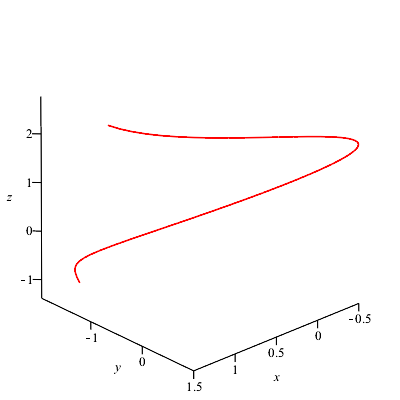
\includegraphics{9_7_VVD_Example}}
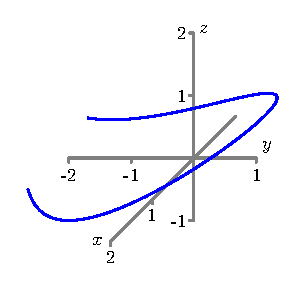
\includegraphics{figures/fig_9_7_activity.eps}
\caption{The position graph for the function in Activity~\ref{A:9.7.7}.}
\label{F:9.7.VVD_Example}
\end{center}
\end{figure}

\end{activity}
\begin{smallhint}

\end{smallhint}
\begin{bighint}

\end{bighint}
\begin{activitySolution}
	\ba
	\item Since acceleration is the derivative of the velocity we have 
\[\va(t) = \vv'(t) = -4\cos(2t)\vi -2\sin(t) \vj + \left(\frac{1}{(1+t)^2}\right) \vk.\]

	\item The position of the object is an antiderivative of the velocity, so 
\[\vr(t) = \int \vv(t) \, dt = \cos(2t) \vi + 2\sin(t) \vj + \left( t - \ln|1+t| \right) \vk + \vC\]
for some constant $\vC$. Since $\vr(0) = \langle 1.5, -1, 0 \rangle$, we have 
\[\langle 1.5, -1, 0 \rangle = \vr(0) = \langle 1, 0, 0 \rangle + \vC\]
and so $\vC = \langle 0.5, -1, 0 \rangle$. Therefore,
\[\vr(t) = (\cos(2t)+0.5) \vi + (2\sin(t)-1) \vj + \left( t - \ln|1+t| \right) \vk.\]
	\item The position $\vr(1) = (\cos(2)+1) \vi + (2\sin(1)-1) \vj + (1-ln(2)) \vk$, velocity $\vv(1) = (-2\sin(2)) \vi + (2\cos(1)) \vj + \left(\frac{1}{2}\right) \vk$, and acceleration vector $\va(1) = (-4\cos(2)) \vi - (2\sin(1)) \vj + \left(\frac{1}{4}\right) \vk$ of the object at time $t=1$ are shown below. 
%\begin{figure}[ht]
\begin{center}
\resizebox{!}{2.0in}{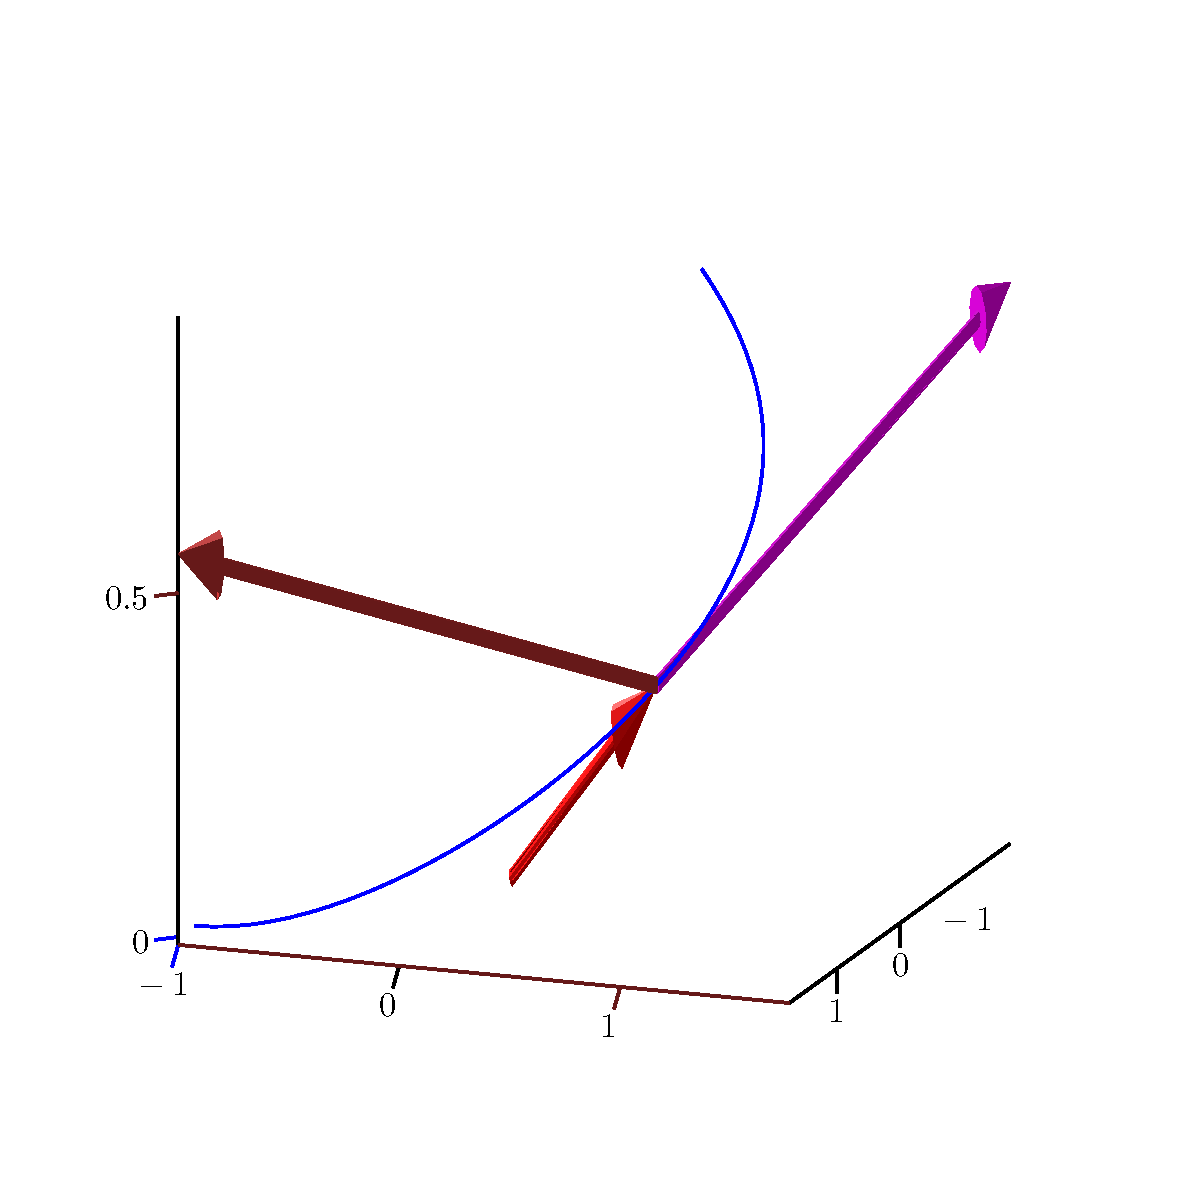
\includegraphics{figures/9_7_Act30_c_sol}}
%\caption{The distance formula in $\R^3$.}
%\label{F:9.1.Distance_3D}
\end{center}
%\end{figure}	
	\item The vector $\vv(1)$ is a direction vector for $\vL(t)$ and so
\[\vL(t) = \vr(1) + t\vv(1) = \langle \cos(2)+1, 2\sin(1)-1, 1-\ln(2) \rangle + t \left\langle -2\sin(2), 2\cos(1), + \frac{1}{2} \right\rangle.\]


	\ea
\end{activitySolution}
\aftera
